\documentclass{article}
\usepackage{graphicx} % Required for inserting images
\usepackage{amsmath}
\usepackage{amssymb}
\usepackage{enumitem}
\usepackage{subfig}

\begin{document}
\begin{center}
\textbf{
{\Large HKN ECE 120 Midterm 3 Worksheet}
}
\end{center} 
\noindent\makebox[\linewidth]{\rule{\linewidth}{0.2pt}}


\section*{Serialized Design (Review)}
\subsection*{Problem 1}
Consider one bit-slice of a full adder.
\begin{enumerate}[label=\alph*.]
    \item How many bits need to be passed between each bit slice? What are they?
    \item If we wanted to serialize this design and add 1 bit at a time, how many D flip-flops would we need to store these signals?
    \item Implement a serialized binary adder, adding 1 bit at a time.
    \item Assume we instead wanted to add 4 bits (1 hexadecimal) at a time. Would any signals be different?
    \item Implement a serialized binary adder, adding 4 bits at a time.
\end{enumerate}


\subsection*{Problem 2}
Consider a serialized circuit that takes a sequence of bits, 1 bit at a time, and outputs the same sequence of bits but is delayed by 2 bits and inverted. For example, assuming inputs and outputs are taken at the start of each clock cycle, if the input is 100101101100, then the output is XX0110100100.
\begin{enumerate}[label=\alph*.]
    \item How many bits do we need to store between each clock cycle?
    \item Implement this circuit using D flip-flops.
    \item Can we also implement this circuit using a shift register?
\end{enumerate}


\subsection*{Problem 3}
In 50 words or less, what are the advantages and disadvantages of serialization over bit-slicing?


\newpage
\section*{Finite State Machines}
\subsection*{Problem 1}

Suppose we wanted to create a Moore FSM that has two outputs $Z$ and $O$. $Z$ is 1 if and only if the input contains three or more consecutive zeroes, and $O$ is 1 if and only if the input contains three or more consecutive ones.

\begin{enumerate}[label=\alph*.]
\item How many unique states do we need for this finite state machine? How many bits do we need to represent all states?
\item Draw a state diagram for this FSM, showing all states used.
\item Create a truth table for this FSM. For unused states, write $X$.
\item Use K-maps or another method to derive next-state expressions for this FSM.
\item Implement this FSM using D flip-flops.
\end{enumerate}

\subsection*{Problem 2}

Suppose we wanted to create a Mealy FSM that represents an elevator in a building with 6 floors, 1 through 6. It takes two clock cycles for the elevator to move between floors. The input is a 3-bit unsigned integer $I_2I_1I_0$ and the output is a single bit $F$ that is 1 when the elevator has reached the correct floor and 0 when it has not. You may assume that the input is always between 1 and 6 (inclusive).

\begin{enumerate}[label=\alph*.]
\item How many unique states do we need for this finite state machine? How many bits do we need to represent all states?
\item Draw a state diagram for this FSM, showing all states used. You may also use comparisons ($=, <, >$). (Hint: it might be helpful to enumerate the states in a way that preserves the 3-bit floor)
\item Create a truth table for this FSM, defining new intermediate variables for your comparisons. For unused states, write $X$.
\item Use K-maps or another method to derive next-state expressions for this FSM.
\item Implement this FSM using D flip-flops and a 3-bit digital comparator, with outputs for $A > B$, $A = B$, and $A < B$. Feel free to use adders, MUXes, buses, or any other component covered earlier in the course.
\end{enumerate}

\newpage
\subsection*{Problem 3}
Taken from HDLBits "Design a Moore FSM"\\
\begin{figure}[!h]
    \centering
    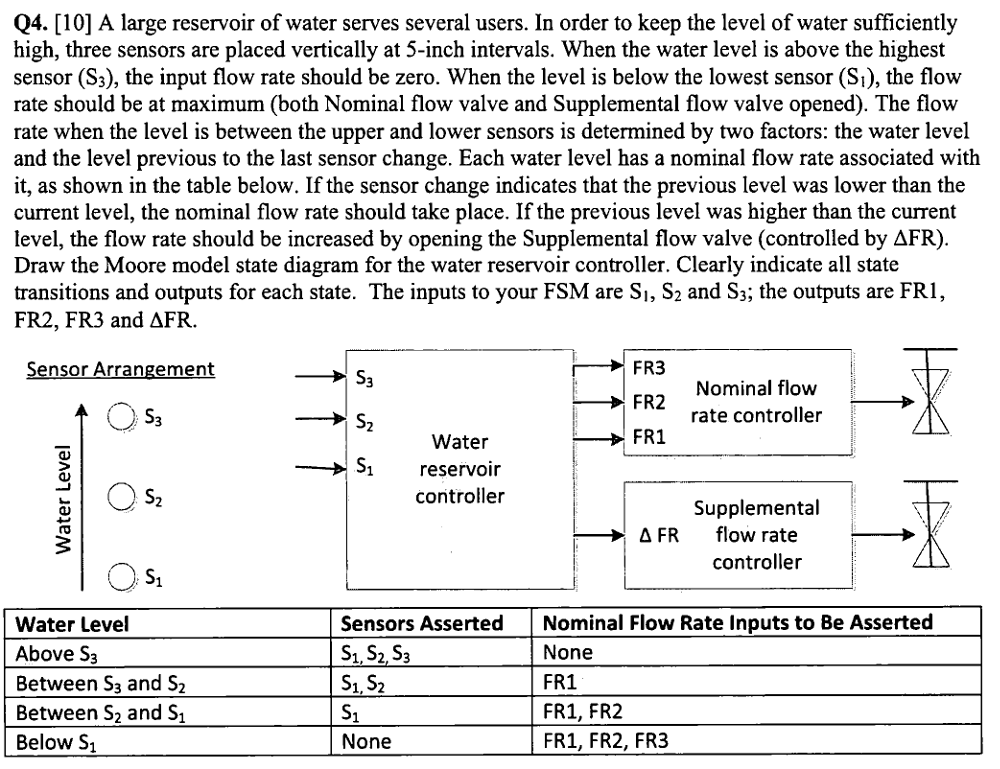
\includegraphics[width=0.7\textwidth]{figures/fsm_q3.png}
\end{figure}


\newpage
\section*{Memory}
\subsection*{Problem 1}

\begin{enumerate}[label=\alph*.]
\item What is memory addressability? What is the difference between memory addressability and a memory address?
\item What is the purpose of the chip select signal in a RAM block?
\item What is the purpose of the write enable signal in a RAM block?
\item Describe the process to read from a RAM block. Detail the signal values:
\item Describe the process to write from a RAM block. Detail the signal values:

\end{enumerate}

\subsection*{Problem 2}
\begin{figure}[!h]
    \centering
    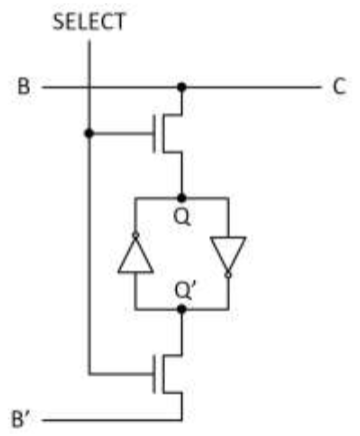
\includegraphics[width=0.3\textwidth]{figures/memory_q2.png}
\end{figure}

\begin{enumerate}[label=\alph*.]
\item What should we apply to Select, B and B’ in order to read the value Q to C?
\item What should we apply to Select, B and B’ in order to hold a value Q?
\item What should we apply to Select, B and B’ in order to write a 0 to Q?
\item What should we apply to Select, B and B’ in order to write a 1 to Q?
\end{enumerate}

\newpage
\subsection*{Problem 3}
\begin{figure}[!h]
    \centering
    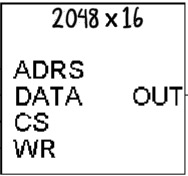
\includegraphics[width=0.3\textwidth]{figures/memory_q1.jpg}
\end{figure}
For each of the combinations below, select and draw those that can be used to build a 2048 x 12 RAM using only the parts given. If not possible, explain why. Assume that logic 0 and 1 signals are available and that the chip select and write enable are active-high.

\begin{enumerate}[label=\alph*.]
\item Two 1024 x 6 RAMs and one 4:1 multiplexer
\item Four 512 x 12 RAMs and a 2:4 priority encoder
\item Two 2048 x 6 RAMs	
\item Four 512 x 3 RAMs and two 4:1 multiplexers
\end{enumerate}


\newpage
\section*{LC-3 ISA}
\subsection*{Problem 1}
Review Questions. Answer for the LC-3 ISA.
\begin{enumerate}[label=\alph*.]
\item How many bits are used to address memory? What is the memory address space?
\item How many bits of data are stored at each memory space/what is the memory addressibility?
\item What is the bus width?
\item How many registers are in the register file? How wide are they?
\item How many other registers are there? How wide are they?
\item How do we control which signals are sent to the system bus?
\end{enumerate}

\subsection*{Problem 2}
Consider the Von Neumann Architecture.
\begin{figure}[!h]
    \centering
    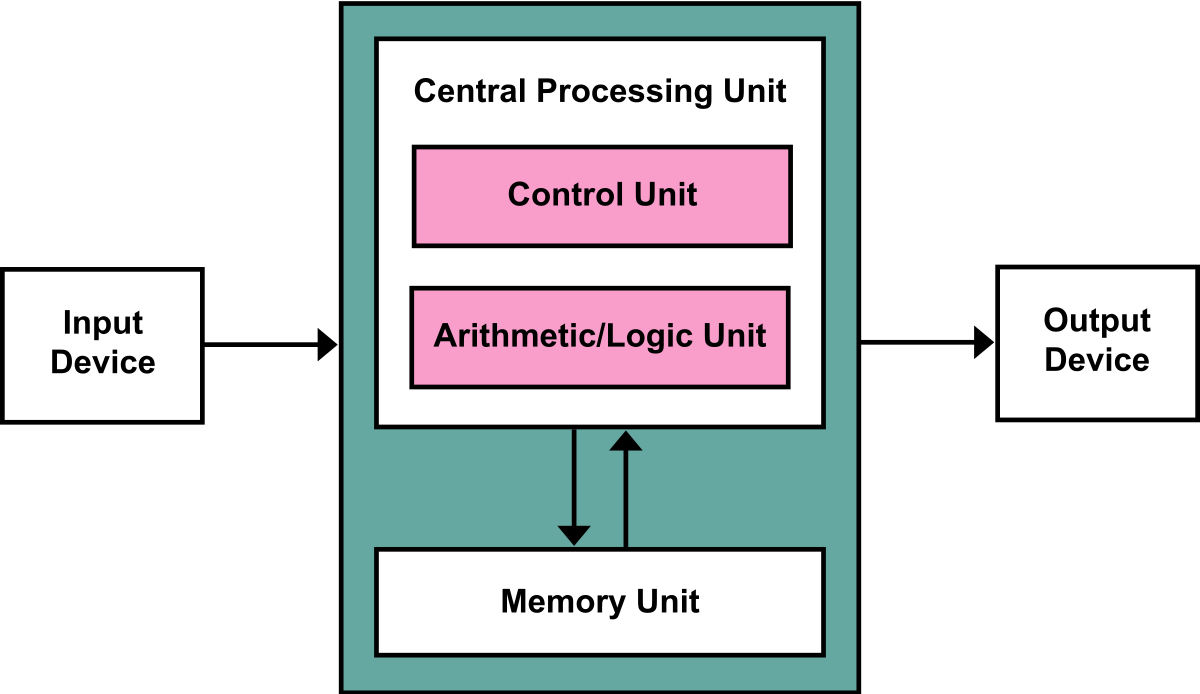
\includegraphics[width=0.7\textwidth]{figures/von_neumann.png}
\end{figure}
\begin{enumerate}[label=\alph*]
\item In 50 words or less, explain the role of the control unit.
\item In 50 words or less, explain the role of the ALU.
\item For the LC-3 ISA, what does the control unit correspond to?
\item For the LC-3 ISA, what are the inputs and outputs?
\end{enumerate}

\newpage
\subsection*{Problem 3}
Tracing LC-3. Refer to Patt and Patel Figure C.2.
\begin{enumerate}[label=\alph*]
\item Write down the control signals for states 18, 33, 35, and 32 in the following tables. Use X for unused signals.

\begin{table}[!h]
\begin{tabular}{|l|l|l|l|l|l|l|l|}
\hline
\textbf{State} & \textbf{LD.BEN} & \textbf{LD.MAR} & \textbf{LD.MDR} & \textbf{LD.IR} & \textbf{LD.PC} & \textbf{LD.REG} & \textbf{LD.CC} \\ \hline
18             &                 &                 &                 &                &                &                 &                \\ \hline
33             &                 &                 &                 &                &                &                 &                \\ \hline
35             &                 &                 &                 &                &                &                 &                \\ \hline
32             &                 &                 &                 &                &                &                 &                \\ \hline
\end{tabular}
\end{table}
\begin{table}[!h]
\begin{tabular}{|l|l|l|l|l|l|l|}
\hline
\textbf{State} & \textbf{GateMARMUX} & \textbf{GateMDR} & \textbf{GateALU} & \textbf{GatePC} & \textbf{MARMUX} & \textbf{PCMUX} \\ \hline
18             &                     &                  &                  &                 &                 &                \\ \hline
33             &                     &                  &                  &                 &                 &                \\ \hline
35             &                     &                  &                  &                 &                 &                \\ \hline
32             &                     &                  &                  &                 &                 &                \\ \hline
\end{tabular}
\end{table}
\begin{table}[!h]
\begin{tabular}{|l|l|l|l|l|l|l|l|}
\hline
\textbf{State} & \textbf{ADDR1MUX} & \textbf{ADDR2MUX} & \textbf{DRMUX} & \textbf{SR1MUX} & \textbf{ALUK} & \textbf{MIO.EN} & \textbf{R.W} \\ \hline
18             &                   &                   &                &                 &               &                 &              \\ \hline
33             &                   &                   &                &                 &               &                 &              \\ \hline
35             &                   &                   &                &                 &               &                 &              \\ \hline
32             &                   &                   &                &                 &               &                 &              \\ \hline
\end{tabular}
\end{table}
\item What are the components of the instruction processing cycle for LC-3? 
\item What does each state correspond to in the instruction processing cycle?
\item Suppose we wanted to make a new state that performs the following operation: $R6 \longleftarrow R6 + \text{PC}$, set CC.
Write down the control signals that are needed and what they should be.

\end{enumerate}

\newpage
\subsection*{Problem 4}
Implementing a new instruction, including control signals.\\\\
We want to implement the following instruction: \\
PC $\longleftarrow$ PC + M[BaseR + PCOffset6] + 1 \\\\
Note: the +1 is to accommodate state 18. \\
Note 2: In the very rare case that you actually read the textbook, pretend Appendix C.6.3 did not exist.\\
\begin{enumerate}[label=\alph*]
\item We know that LC-3 has one unused opcode, the opcode 1101. When this opcode is decoded, suppose that the LC-3 FSM enters state 48 (110000). How many FSM states will this instruction need? What will each state do? Assign them in the 48-55 range.
\item How will each instruction transition to each other state? Draw a state diagram.
\item Using K-maps or another method, write an expression for the next state transition. (Hint: $S_5S_4S_3 = 110$, and memory ready is the signal $R$. you can work with the 4 bits $RS_2S_1S_0$)
\item Using a similar table as in Problem 3a, write down the control signals for each state.
\item Trace through your instruction with the following instruction: \\
1101 000 101 000111 \\
Assume PC = x3001, R5 = x2000, and M[x2007] = x8EED. \\
What is PC after the instruction completes and before the next execution of state 18?

\end{enumerate}

\newpage
\section*{LC-3 Assembly}
\subsection*{Problem 1}
\begin{figure}[!h]
    \centering
    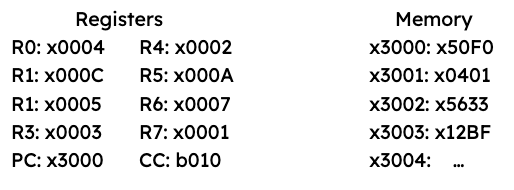
\includegraphics[width=1\textwidth]{figures/lc3_q1.png}
\end{figure}

\begin{figure}[!h]
    \centering
    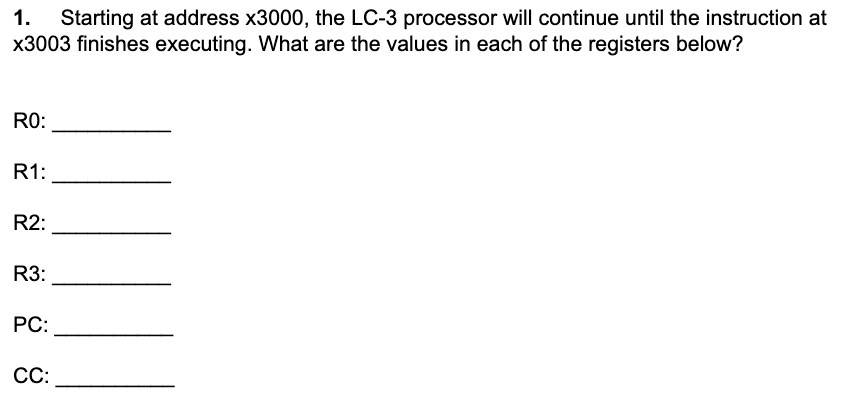
\includegraphics[width=1\textwidth]{figures/lc3p1p3.png}
\end{figure}


\begin{figure}[!h]
    \centering
    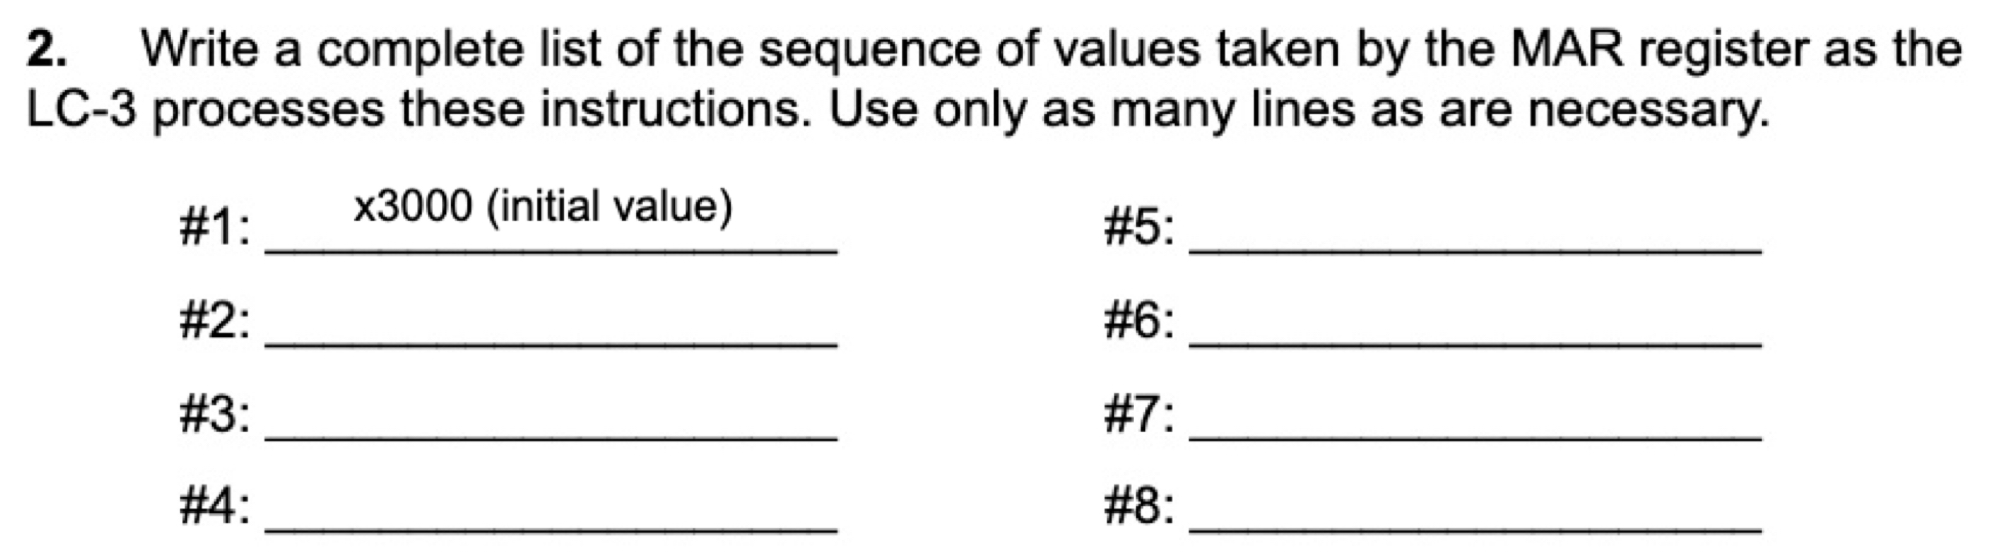
\includegraphics[width=1\textwidth]{figures/lc3_q1p2.jpg}
\end{figure}

\newpage
\subsection*{Problem 2}
Write an LC-3 Assembly program that compares two numbers in R2 and R3 and puts the larger number into R1. If the numbers are equal, then R1 is set equal  to 0. Use as many lines as necessary.
\begin{figure}[!h]
    \centering
    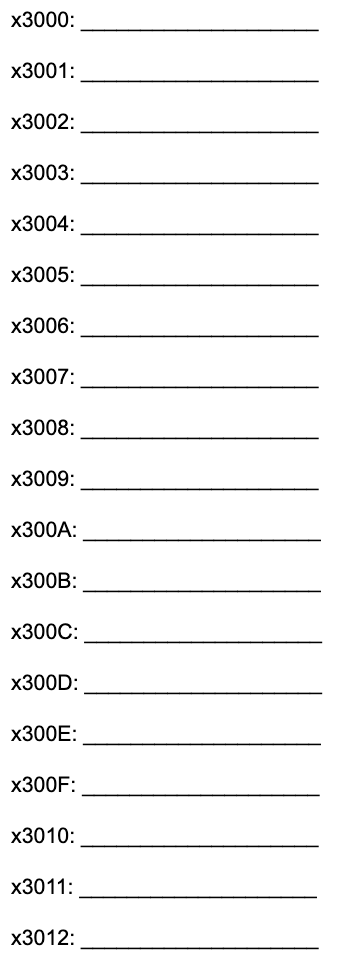
\includegraphics[width=0.5\textwidth]{figures/lc3_q2.png}
\end{figure}

\newpage
\subsection*{Problem 3}
Write two LC-3 Assembly programs that executes a bitwise OR operation and a bitwise XOR operation respectively on R4 and R5 and puts the result in R1. How might you extend these to support NOR and XNOR?
\begin{figure}[!h]
    \centering
    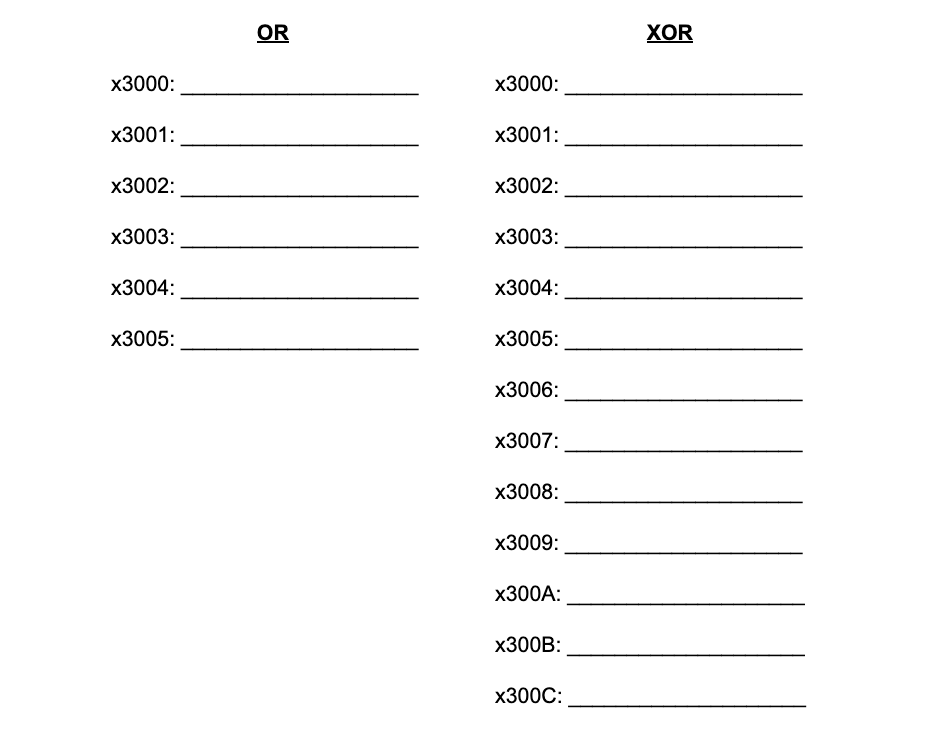
\includegraphics[width=1\textwidth]{figures/lc3_q4.png}
\end{figure}

\newpage
\subsection*{Problem 4}
\begin{enumerate}[label=\alph*.]
\item Assuming LC-3 now has 32 registers, we want to increase the number of registers that we can specify in the LC-3 ADD instruction to 32. Is there a problem with this? Explain.
\item A memory's addressibility is 64 bits. What does that tell you about the size of the MAR and MDR, given a 64-bit ISA and $2^{20}$ memory locations?
\item Say we have a memory consisting of 256 locations, and each location contains 16 bits. How many bits are required for the address for a byte-addressable system? Explain.
\end{enumerate}

\end{document}

